\subsection{Fast Eagle}
  \subsubsection{Definición y objetivos}
    \paragraph{Éste módulo es el encargado de brindar la información procesada al usuario a través de una página de internet. Es el módo visual que los usuarios finales tendrán para poder interactuar con el ecosistema Ambienta2MX.}
    \paragraph{Se presenta cómo un módulo web que consumirá la información procesada y almacenada por las cuatro bases (MX1,MX2,MX3,MX4) y la base de soporte (Places).}
    \paragraph{La principal función es la de consulta y visualización de datos. Es la capa más expuesta y visual de Ambienta2MX ya que es la que tendrá interacción directa con usuarios no técnicos, sin embargo, contará con los procesos necesarios para poder extraer información de las demás plataformas en formatos convencionales cómo JSON o CSV para uso posterior del usuario.}
  \subsubsection{Alcances}
    \paragraph{Interactúa de forma directa con el bloque \textbf{\emph{Cute Bunny}}, que forma parte de la segunda capa de exposición de datos de Ambienta2MX. Se comunica con los demás módulos mediante servicios de tipo REST que funcionan bajo el patrón de convención sobre configuración\cite{8}, brindando así una gran compatibilidad con éstos además de disminuir el tiempo de desarrollo debido a que no es necesario generar código único y se opta por la reutilización de éste además de apoyarse con el uso de bibliotecas que siguen el mismo método de trabajo.}
    \paragraph{Friendly Dolphin sólo puede ser visto como una herramienta de consulta, no podrá ser visto cómo un utensilio de análisis de datos climatológicos, es por ello que muestra la información en mapas, gráficas y detalles de la consulta.}
  \subsubsection{Restricciones}
    \paragraph{Éste módulo se ve limitado por la API de Google Maps para la visualización de la información, ya que las consultas resultan limitadas en su versión gratuita, sin embargo, la cantidad es suficiente para demostrar la aplicación de los datos en una herramienta de visualización. Las restricciones estan definidas a 25,000 solicitudes por día y limitada a un segundo por petición o usuario.}
    \paragraph{La vista también cuenta con cierta limitantes, sólo podrá ser visualizada en navegadores con Internet Explorer 11+, Mozilla Firefox 20+ y Google Chrome 20+}
  \subsubsection{Arquitectura}
    \paragraph{Friendly Dolpin contará con varios procesos y módulos a ser desarrollados. Éste módulo se desarrollará usando tecnologías cómo HTML, Javascript y CSS, además de contar con un ciclo continuo de desarrollo usando herramientas de apoyo cómo Yeoman, Gulp para el maquetado y gestión de tareas comunes en projectos de tipo web.}
    \paragraph{Se hará uso del servidor interno que ofrece Gulp junto con las tareas y gestión de bibliotecas de terceros. En cuanto al desarrollo de los estilos necesarios para las vistas se implementará Bootstrap cómo maquetado CSS y finalmente el manejo de vistas, peticiciones y lógica dentro del navegador de los clientes se implementará un patrón de tipo SPA (Single Page Application)\cite{36} desarrollado por el equipo de trabajo.}
    \begin{figure}[b!]
      \centering
        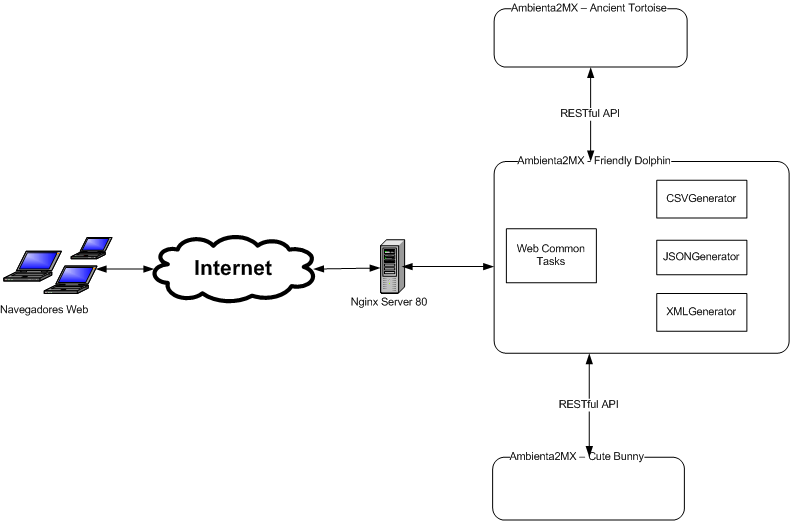
\includegraphics[width=22.5cm,height=12cm]{./images/DiagramaFriendlyDolphin.png}
      \caption{Diagrama General de Friendly Dolphin}
    \end{figure}
  \subsubsection{Factibilidad}   
    \paragraph{Se decidió cambiar de framework en las vistas, se quitó la implementación de EmberJs del proyecto y se optó por seguir la ideología que éste tiene, considerando un patrón SPA mínimo ya que el framework antes mencionado contaba con demasiadas características que no iban a ser implementadas sin embargo el framework hace uso de estas.}
    \paragraph{Se optó por seguir esa ideología brindando la flexibilidad necesaria que consideró el equipo de trabajo para cumplir con el objetivo de tener una página dinámica que convive con los demás módulos de Ambienta2MX.}
  \subsubsection{Pruebas y Capturas de pantalla}
    \paragraph{Para este módulo se realizaron pruebas funcionales indicando el flujo básico de información que un usuario común seguiría. Las pantallas básicas se muestran a continuación y la información de las pruebas pueden ser visualizadas en el anexo en este documento.}
    \begin{figure}[b!]
      \centering
        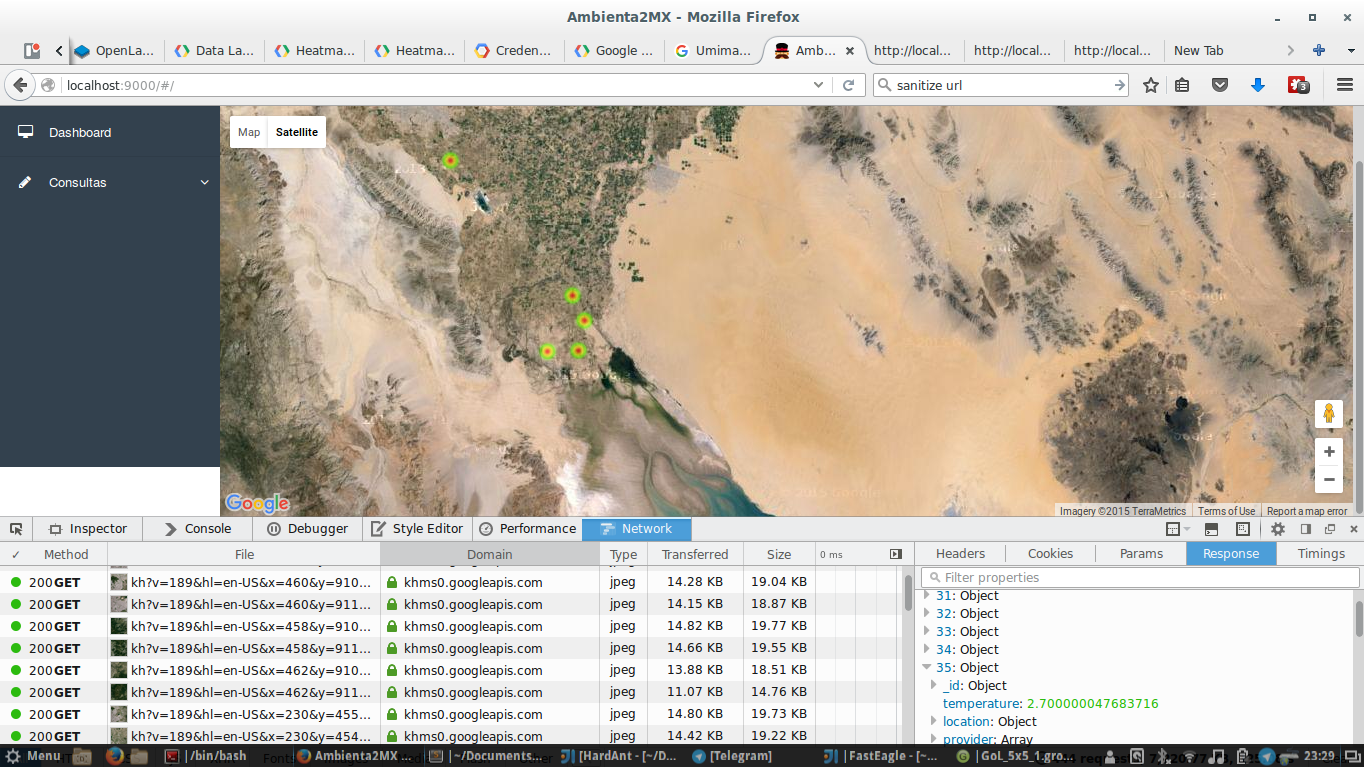
\includegraphics[width=22.5cm,height=12cm]{./images/CapturaFriendlyDolphin}
      \caption{Mapas de Calor, Friendly Dolphin}
    \end{figure}
    \begin{figure}[b!]
      \centering
        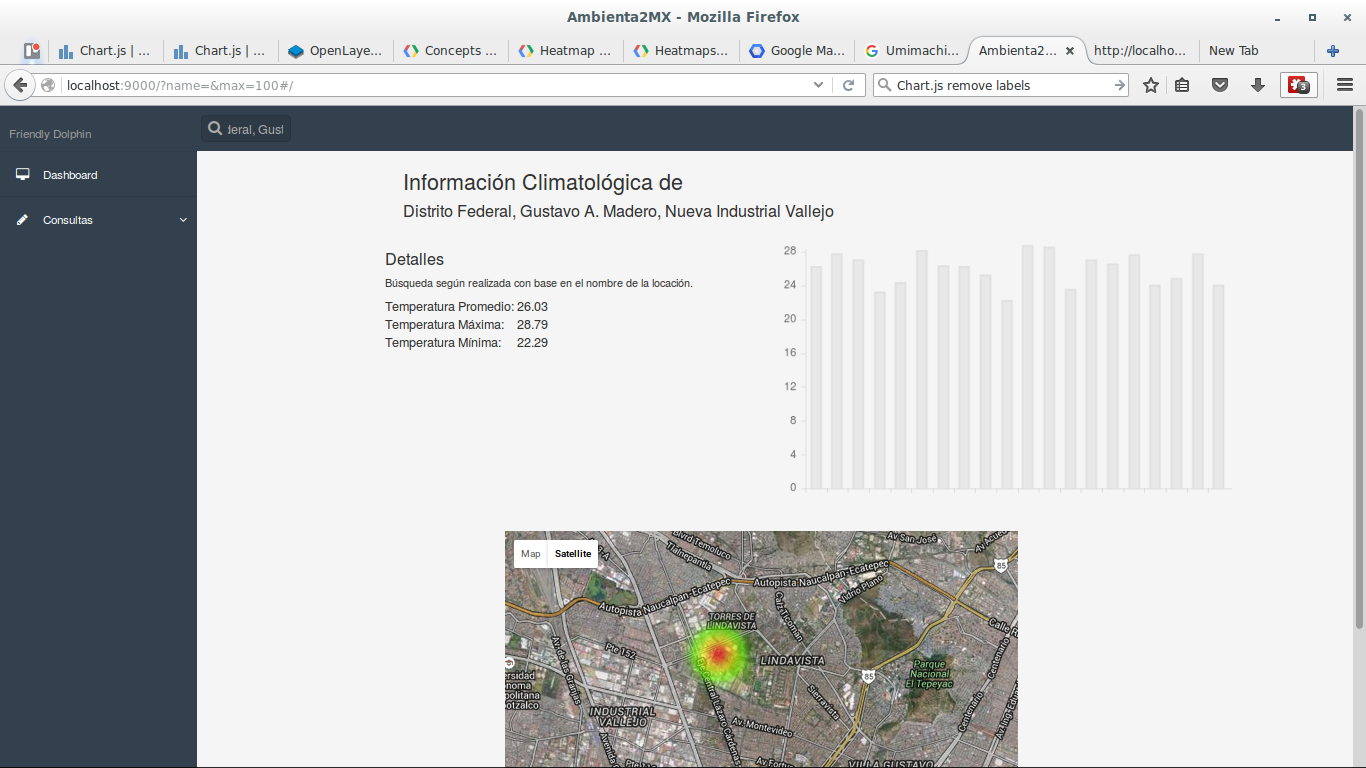
\includegraphics[width=22.5cm,height=12cm]{./images/CapturaFriendlyDolphin2}
      \caption{Tablas e información de clima, Friendly Dolphin}
    \end{figure}